\documentclass[12pt,a4paper]{article}

%%%%%%%%%%%%%%%%%%%%%%%%% packages %%%%%%%%%%%%%%%%%%%%%%%%
\usepackage{tikz}
\usepackage{verbatim}
\usepackage{graphicx}
\usepackage{subcaption}
\usetikzlibrary{arrows,shapes}
\usepackage{amsmath}
\usepackage{amssymb}
\usepackage{physics}
\usepackage{amsthm}
\usepackage{amsmath}
\usepackage{amsfonts}
\usepackage{graphicx}
\usepackage[all]{xy}
\usepackage{tikz}
\usepackage{verbatim}
\usepackage[left=2cm,right=2cm,top=3cm,bottom=2.5cm]{geometry}
\usepackage{hyperref}
\usepackage{caption}
\usepackage{subcaption}
\usepackage{psfrag}

%%%%%%%%%%%%%%%%%%%%% students data %%%%%%%%%%%%%%%%%%%%%%%%
\newcommand{\student}{Your full name here!}
\newcommand{\course}{Course name goes here!}
\newcommand{\assignment}{Put a number here!}

%%%%%%%%%%%%%%%%%%% using theorem style %%%%%%%%%%%%%%%%%%%%

\newtheorem{thm}{Theorem}
\newtheorem{lem}[thm]{Lemma}
\newtheorem{defn}[thm]{Definition}
\newtheorem{exa}[thm]{Example}
\newtheorem{rem}[thm]{Remark}
\usepackage{braket}
\newtheorem{coro}[thm]{Corollary}
\newtheorem{quest}{Question}[section]

%%%%%%%%%%%%%%  Shortcut for usual set of numbers  %%%%%%%%%%%

\newcommand{\N}{\mathbb{N}}
\newcommand{\Z}{\mathbb{Z}}
\newcommand{\Q}{\mathbb{Q}}
\newcommand{\R}{\mathbb{R}}
\newcommand{\C}{\mathbb{C}}
\newcommand{\tens}[1]{%
	\mathbin{\mathop{\otimes}\limits_{#1}}%
}

%%%%%%%%%%%%%%%%%%%%%%%%%%%%%%%%%%%%%%%%%%%%%%%%%%%%%%%555
\begin{document}
\pgfdeclarelayer{background}
\pgfsetlayers{background,main}


%%%%%%%%%%%%%%%%%%%%%%% title page %%%%%%%%%%%%%%%%%%%%%%%%%%
\thispagestyle{empty}
\begin{center}
\textbf{AFRICAN INSTITUTE FOR MATHEMATICAL SCIENCES \\[0.5cm]
(AIMS RWANDA, KIGALI)}
\vspace{1.0cm}
\end{center}

%%%%%%%%%%%%%%%%%%%%% assignment information %%%%%%%%%%%%%%%%
\noindent
\rule{17cm}{0.2cm}\\[0.3cm]
Name: Sittana Osman Afifi Mohamedelmubarak \hfill  ch 2\\[0.1cm]
Zero-Knowledge proofs: Implementation of the Graph Isomorphism Protocol  \hfill Date: \today\\
\rule{17cm}{0.05cm}
\vspace{1.0cm}

\section{Graph isomorphism}
\begin{defn}[Graph \cite{gross2003handbook:5}] An undirected graph consists of a set of vertices (nodes) $V$ and a set of edges $E$.\\
Two nodes $u$ and $v$ are said to be adjacent if there is an edge $(u,v) \in E$.
\end{defn}
We can describe graph using its adjacency matrix which is a square matrix $M_{n\times n}$, with $m_{ij}=1 $ if $(i,j)\in E$ and $0$ otherwise.     
\begin{defn}
Let $V(G)$, $E(G)$ denote the vertex set and edge set of a graph $G$ respectively. Then, a pair of graphs $(G_0, G_1)$ are \textbf{isomorphic} (denoted $G_0 \cong G_1$) if there exists a bijective map $\Pi:V(G_0)\longmapsto V(G_1)$such that $\forall x,y \in V(G_0), (x,y)\in E(G_0)$ if and only if $(\Pi(x)\Pi(y))\in E(G_1)$. The permutation $\Pi$ is called an isomorphism.\cite{lec-notes1:3}
\end{defn}
In other words: two graphs are said to be isomorphic if after we relabel vertices in one graph we get the other graph (with the same adjacency matrix).
\begin{exa}
 Two isomorphic graphs with their corresponding adjacency matrices.
\begin{figure}[h!]
	\centering
	\begin{subfigure}[b]{.29\linewidth}
		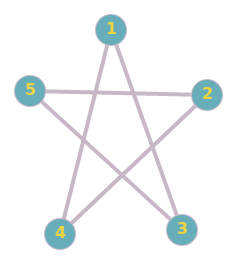
\includegraphics[width=\linewidth]{ex1_1.png}
		\caption{$G_0$.}
	\end{subfigure}
	\begin{subfigure}[b]{.24\linewidth}
		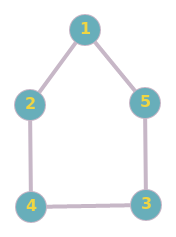
\includegraphics[width=\linewidth]{ex1_2.png}
		\caption{$G_1$.}
	\end{subfigure}
	\caption{Two isomorphic graphs.}
	\label{fig:Two isomorphic graphs}
\end{figure}
\begin{table}[!htb]
	%\caption{Crossponding ajacency matrix }
	\begin{minipage}{.5\linewidth}
		
		\centering
		\begin{tabular}{|c|c|c|c|c|c|}
			\hline 
			& \textbf{1} & \textbf{2} & \textbf{3} & \textbf{4} & \textbf{5} \\ 
			\hline 
			\textbf{1} & 0 & 0 & 1 & 1 & 0 \\ 
			\hline 
			\textbf{2} & 0 & 0 & 0 & 1 & 1 \\ 
			\hline 
			\textbf{3} & 1 & 0 & 0 & 0 & 1 \\ 
			\hline 
			\textbf{4} & 1 & 1 & 0 & 0 & 0 \\ 
			\hline 
			\textbf{5} & 0 & 1 & 1 & 0 & 0 \\ 
			\hline  
		\end{tabular} 
	\caption{adjacency matrix of $G_0$}
	\end{minipage}%
	\begin{minipage}{.5\linewidth}
		\centering

		\begin{tabular}{|c|c|c|c|c|c|}
			\hline 
			& \textbf{1} & \textbf{2} & \textbf{3} & \textbf{4} & \textbf{5} \\ 
			\hline 
			\textbf{1} & 0 & 1 & 0 & 0 & 1 \\ 
			\hline 
			\textbf{2} & 1 & 0 & 0 & 1 & 0 \\ 
			\hline 
			\textbf{3} & 0 & 0 & 0 & 1 & 1 \\ 
			\hline 
			\textbf{4} & 0 & 1 & 1 & 0 & 0 \\ 
			\hline 
			\textbf{5} & 1 & 0 & 1 & 0 & 0 \\ 
			\hline 
		\end{tabular}
			\caption{adjacency matrix of $G_1$}
	\end{minipage} 
\end{table}

In Figure \ref{fig:Two isomorphic graphs} $G_1$ is obtained, by relabeling the vertices of $G_0$ according to the following permutation: (1, 4, 5, 2, 3). This means that Node 3 in $G_0$ becomes Node 5 in $G_1$, Node 4 becomes Node 2. 
\end{exa}
\subsection{Graph Isomorphism based Zero-Knowledge Proofs}
Suppose we have two isomorphic graphs $G_0$ and $G_1$ and $G_1=\Pi(G_0)$, with limited messages between the prover ($P$) and verifier($V$), $P$ wants to prove to $V$ he knows the secret $\Pi$ without showing him what is $\Pi$ exactly.
In the previous example, we can see that it is easy to show if two graphs are isomorphic or not but this process isn’t always simple; suppose we have two graphs each with $10$ vertices and $28$ edges, such as the graphs in Figure \ref{fig:Two isomorphic graphs has 10 vertices and 28 edges}:
\begin{figure}[h!]
	\centering
	\begin{subfigure}[b]{.39\linewidth}
		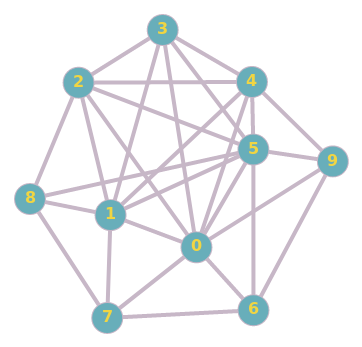
\includegraphics[width=\linewidth]{ex2_1.png}
		\caption{$G_0$.}
	\end{subfigure}
	\begin{subfigure}[b]{.39\linewidth}
		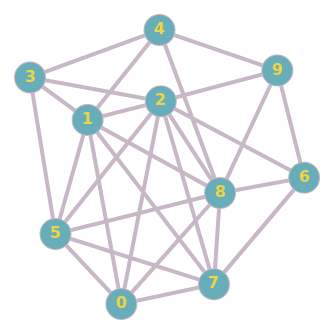
\includegraphics[width=\linewidth]{ex2_2.png}
		\caption{$G_1$.}
	\end{subfigure}
	\caption{Two isomorphic graphs.}
	\label{fig:Two isomorphic graphs has 10 vertices and 28 edges}
\end{figure}\\
Then ZKP can provide a protocol that $P$ can prove to $V$ he knows the secret $\Pi$ without revealing $\Pi$ itself.\\
The protocol is done by applying a random permutation ($\varphi$) on $G_0$ by $P$, with: $$H=\varphi(G_0)$$ and the honest prover has to be able to find a permutation such that he could transform $H$ to either $G_0$ or $G_1$.(i.e to prove $H\cong G_0$ or $H\cong G_1$)\\
\subsection{ Zero-Knowledge Protocol for Graph Isomorphism}
We have two graphs known by both parties $G_0$ and $G_1$ such that they have $n$ vertices, define $S_n$ as a set of permutations of $n$ elements.\\   
The protocol proceeds by the following:\cite{lec-notes1:3}\\
\textbf{Input}: pair of graphs $(G_0,G_1)$
\begin{enumerate}	
	\item
	\begin{enumerate}
\textbf{prover} chooses random permutation $\sigma$ from $S_n$, and sends $H=\sigma(G_0)$.
\end{enumerate}
	\item
\begin{enumerate}
\textbf{verifier}  chooses $ch$ randomly from $\{0,1\}$ and sends it to the prover.
\end{enumerate}
	\item
\begin{enumerate}
\textbf{prover} if $ch=0$: then sends $\varphi=\sigma$ else sends $\varphi=\sigma \circ \Pi^{-1}$.
\end{enumerate}
	\item
\begin{enumerate}
\textbf{verifier} output \underline{ACCEPT} if $H=\varphi(G_{ch})$ else output is \underline{REJECT}.\\

\end{enumerate}
\end{enumerate}
\subsection{graph isomorphism (GI) decision problem}
\begin{defn}[graph isomorphism (GI) decision problem \cite{goldreich2007foundations:17}]
\textit{Input}: pair of two finite graphs ($G_0 , G_1$).\\
\textit{Output}: ACCEPT if and only if they are isomorphic.\\
Complexity can be measured in the number of vertices.
\end{defn}
\subsubsection{The complexity of GI \cite{goldreich2007foundations:17}}
If we have two graphs and we want to check whether they are isomorphic or not; the brute force algorithm is to apply all possible permutation in $S_n$ but this run in $n!$ and it’s slower than any exponential algorithm.\\
There is a petter algorithm but not in polynomial-time, because no polynomial-time algorithm yet is known to solve it (if it was in P, then there is no need to apply ZKP; the verifier can check if graphs are isomorphic).\\  
Moreover, GI also isn't considered to be NP-complete, This put GI in  intermediate complexity problems (neither P nor NP-complete). 
In L{\'a}szl{\'o} Babai’s paper \cite{babai2016graph:16} according to  \textbf{Corollary, 1.1.2} GI can be solved in quasipolynomial time and it’s run in $O(exp(log(n)^c))$
\begin{thm}\cite{goldreich2007foundations:17}\\
The above protocol satisfies completeness, soundness $\frac{1}{2}$, and zero-knowledge.	
\end{thm}
\textbf{Proof}\\
\textbf{Completeness.}
Completeness is quite straight forward, here we are dealing with honest prover $G_0\cong G_1$ who knows $\Pi$, the verifier will check $\varphi$ for both possible cases:
\begin{enumerate}	
\item
\begin{enumerate}
($ch=0$): from step (1) $P$ calculates $H=\sigma(G_0)$ and he should find a bijective map from $H$ to $G_0$:\\
it's clear that $\varphi = \sigma$ because $\sigma(G_0)=\sigma(G_0$
\end{enumerate}
	\item
	\begin{enumerate}
($ch=1$): $P$ has to find a map from $H$ to $G_1$ or to show that $H\cong \varphi(G_1)$:\\
		We know that:
\begin{equation}
G_1=\Pi(G_0)\label{eq:1}
\end{equation}
\begin{equation}
H=\sigma(G_0)\label{eq:2}
\end{equation}
After we comibne  equation \ref{eq:1} and equation \ref{eq:2} :\\
		$$H=\sigma (\Pi^{-1}(G_1))$$
		$$H=(\sigma \circ 
		\Pi^{-1})(G_1)$$
		So $$\varphi=\sigma \circ \Pi^{-1}$$
The $V$ has to check that $H\cong \varphi(G_1)$ :\\
$$\varphi(G_1)=\sigma \circ \Pi^{-1}(G_1)=(\sigma \circ \Pi^{-1} \circ \Pi )(G_0)=H$$
	\end{enumerate}
\end{enumerate}
As we see if the prover knows $\Pi$ he can always return the correct permutation.\\
\textbf{Soundness $\frac{1}{2}$.}
For any prover $P^*$ such that $G_0 \ncong G_1$ interacting with an honest verifier $V^*$, then $P^*$ must submit some $\varphi$ to the verifier, $P^*$ can do something like:
\begin{enumerate}
	\item 
	\begin{enumerate}
choose random $\varphi$.
	\end{enumerate}
\item
\begin{enumerate}
pick random $H$ and send it to $V$.
\end{enumerate}
\end{enumerate}
Since $G_0\ncong G_1$ then $H$ such is isomorphic to  $G_0$ or  $G_1$, so whatever prover does, after it sends $H$, $H$ cannot be isomorphic to both $G_0$ and $G_1$.\\
So whatever happens, honest verifier always has at least $1/2$ chance to choose $b$ that fails the prover, so:
$$Pr[P^* \text{ convinces } V \text{ that }G_0 \cong G_1]\leq 1/2$$
If we want to decrease the soundness to be negligible we have to repeat the verification procedure sufficiently many times, if we repeate it $n$ times it will be soundness with $2^{-n}$ which is smaller than any polynomial-time algorithm.

\textbf{zero-knowledge.}
We want to show that there exists a polynomial-time simulator $S$ such that if $G_0$ and  $G_1$ are isomorphic then for an honest prover and for every verifier $V^*$:
\begin{equation}
\text{Distribution of transcript }(P,V^*)=\text{Distribution of transcript } S(G_0,G_1,V^*) 
\label{eq:3}
\end{equation}
\textit{How $S$ works:}
\begin{enumerate}	
	\item
	\begin{enumerate}
$S_n \longleftarrow $ random permutation from $S_n$. 
\end{enumerate}
\item
\begin{enumerate}
$b \longleftarrow$ random bit from $\{0,1\}.$.
\end{enumerate}
\item
\begin{enumerate}
$H=\sigma (G_b)$.
\end{enumerate}
\item
\begin{enumerate}
Send $H$ to $V^*$ to get $ch$.
\end{enumerate}
\item
\begin{enumerate}
If $ch=b$, output $\sigma$ and return the transcript, else loop.
\end{enumerate}
\end{enumerate}
Now we want to show equation \ref{eq:3}  is satisfied:\\
First: the transcript is \{$H,ch(H,V^*),\sigma$\} where $H$ is a result of applying a random permutation on $G_0$ (same as a result of applying a random permutation on $G_1$), $ch$ was generated by $V^*$ from $H$ and $\sigma$ is a random permutation from $S_n$.\\
In the simulator, the distribution is generated in the same way, only there is always probability $\frac{1}{2}$ the simulator loop. But this probability (Pr[$b\neq ch$])  is independent of $H$ so it doesn’t change the distribution of transcripts.\\
Then we want to show is a polynomial-time:\\
Let $k$ be the number of loops, we want to show that $S$ is polynomial-time by calculating the expected value of $k$:\\
When $k=1$ : $E[k]=1/2$\\
When $k=2$ : $E[k]=1/4$\\
When $k=3$ : $E[k]=1/8$ and so on \\
But this is a geometric distribution:
$$P(X = x) = q^{x-1}p$$ where $q = 1 - p$ 
With $E[k]=\sum_{i=1} i*pr(k=i) =\frac{1}{p}=2$\\
Since the expected value of $k$ while $k$ is the number of loops is 2, then $S$ is polynomial-time. 



\bibliography{refer}
\bibliographystyle{ieeetr} 
\end{document}